\documentclass[10pt, a4paper]{article}

%%%%%%%%%%%%%%
%  Packages  %
%%%%%%%%%%%%%%


\usepackage{page_format}
\usepackage{special}
\usepackage{hyperref}
\usepackage[compat=1.1.0]{tikz-feynman}
\input{math_func}

% References
\usepackage{biblatex}
\addbibresource{ref.bib}


%%%%%%%%%%%%
%  Colors  %
%%%%%%%%%%%%
% ! EDIT HERE !
\colorlet{chaptercolor}{red!70!black} % Foreground color.
\colorlet{chaptercolorback}{red!10!white} % Background color


%%%%%%%%%%%%%%
% Page titre %
%%%%%%%%%%%%%%
\title{Homework 2} % Title of the assignement.
\author{\PA} % Your name(s).
\teacher{Bindiya Arora and Dan Wohns} % Your teacher's name.
\class{Quantum Mechanics} % The class title.

\university{Perimeter Institute for Theoretical Physics} % University
\faculty{Perimeter Scholars International} % Faculty
%\departement{<Departement>} % Departement
\date{\today} % Date.


%%%%%%%%%%%%%%%%%%%%%%
% Begin the document %
%%%%%%%%%%%%%%%%%%%%%%
\begin{document}

% Make the title page.
\maketitlepage

% Make table of contents
\maketableofcontents

% Assignment starts here ----------------------------
\section{Two real scalars}

\begin{enumerate}
    \item[(a)] We are considering here perturbative results in the quantum field theory of two interacting real massive scalars $\varphi$, $\Phi$ with respective masses $m$ and $M$. The lagrangian density describing this theory is 
    \begin{align*}
        \mathcal{L} = \dfrac{1}{2}(\partial_\mu \varphi)^2 - \dfrac{1}{2} m^2 \varphi^2  + \dfrac{1}{2}(\partial_\mu \Phi)^2 - \dfrac{1}{2} M^2 \Phi^2 - \frac{g}{2! 1!} \Phi \varphi^2
    \end{align*}
    where $g$ descrives the coupling of the fields and is the parameter of our perturbative expansion. The position-space Feynman rules for perturbative computation of the interacting vacuum $\ket{\Omega}$ n-point functions $\bra{\Omega}T\varphi(x_1) \cdots \Phi(x_k) \cdots  \Phi(x_n)\ket{\Omega}$ for this theory are summed up graphically below:\\[0.3cm]
    \begin{minipage}{0.45\textwidth}
        \begin{center}
        \begin{tikzpicture}
            \begin{feynman}
              % Vertex with a label
              \vertex[label={[shift={(1cm, 0cm)}]right:$-ig \int \text{d}^4x$}] (v);
              \vertex[label={[shift={(0cm, 0.1cm)}]above:$x$}] (v);
              % External legs
              \vertex [left=of v] (a);
              \vertex [above right=of v] (b);
              \vertex [below right=of v] (c);
              \fill (v) circle (2pt);
              % Dashed line
              \diagram* {
                (a) -- [dashed] (v),
                (v) -- (b),
                (v) -- (c),
              };
            \end{feynman}
          \end{tikzpicture}
        \end{center}
    1. Every vertex in a diagram is associated to a four-position variable $x$. Its contribution to the symbolic representation of the amplitude is the integral $-ig \int \text{d}^4x$ acting on the propagators from the $x$ vertex to other vertices. \\[0.3cm]
    3. Divide the amplitude by the symmetry factor of the diagram $S = 2/W$ where $W$ is the number of wick contraction producing the same symbolic diagram expression. $S$ is computed graphically as the order of the fixed end-points automorphism group of the diagram.
    \end{minipage}%
    \hspace{0.3cm}
    \begin{minipage}{0.45\textwidth}
        \begin{center}
        \begin{tikzpicture}
            \begin{feynman}
                % Vertex with a label
                \vertex[label={[left=of v]:$x$}];
                \vertex[label={[shift={(0cm, 0cm)}]right:$y$}];
                \vertex[label={[shift={(-0.8cm, 0.1cm)}]above:$\Delta_{F}^{M}(x-y)$}];
                \vertex[label={[shift={(-0.8cm, -0.9cm)}]above:$1$}];
                % External legs
                \vertex [left=of v] (a);
                \vertex [below=1cm of v] (c); 
                \vertex [below=1cm of a, label={left:$x_1$}] (d); % Adjust the vertical position here

                \fill (a) circle (2pt);
                \fill (v) circle (2pt);
                \fill (d) circle (2pt);

        
                % Dashed line
                \diagram* {
                  (a) -- [dashed] (v),
                  (c) -- [dashed] (d),
                };
              \end{feynman}
          \end{tikzpicture}
        \begin{tikzpicture}
            \begin{feynman}
                % Vertex with a label
                \vertex[label={[left=of v]:$x$}];
                \vertex[label={[shift={(0cm, 0cm)}]right:$y$}];
                \vertex[label={[shift={(-0.8cm, 0.1cm)}]above:$\Delta_{F}^{m}(x-y)$}];
                \vertex[label={[shift={(-0.8cm, -0.9cm)}]above:$1$}];
                % External legs
                \vertex [left=of v] (a);
                \vertex [below=1cm of v] (c); 
                \vertex [below=1cm of a, label={left:$x_1$}] (d); % Adjust the vertical position here

                \fill (a) circle (2pt);
                \fill (v) circle (2pt);
                \fill (d) circle (2pt);

        
                % Dashed line
                \diagram* {
                  (a) -- (v),
                  (c) -- (d),
                };
              \end{feynman}
          \end{tikzpicture}
        \end{center}
          2. Each vertex is the source of two full lines and a dashed line free Klein-Gordon respectively representing a $\varphi$ Feynman propagator $\Delta^m_F(x-y)$ and  a $\Phi$ Feynman propagator $\Delta^M_F(x-y)$ between points $x$ and $y$ (vertices or external points $x_1\cdots x_n$ of the expanded n-point function). Each edge of the diagram is symbolically represented as a multiplication by its associated Feynman propagator. In scalar field theory the external points contribute a trivial factor of $1$ to the amplitude of the diagram. 
    \end{minipage}
    
    \item[(b)] The three-point function $G(x, y, z)  = \bra{\Omega}T \Phi(x)\varphi(y)\varphi(z)\ket{\Omega}$ has no $O(1)$ contributions because the number of contracted fields is odd at this order and no full Wick contractions can be formed: the vacuum is anihilated. At $O(g)$, we have the diagrams\\
    \begin{minipage}{0.45\textwidth}
        \begin{center}
            \begin{tikzpicture}[baseline=(current bounding box.center)]
                \begin{feynman}
                    % Vertex with a label
                    \vertex[label={[left=of v]:$x$}];
                    \vertex[label={[shift={(0cm, 0cm)}]right:$w$}];
                    \vertex[label={[shift={(-0.8cm, 0.1cm)}]above:$\Delta_{xw}^{M}$}];
                    % External legs
                    \vertex [left=of v] (a);
                    \vertex [right=of v, label={[shift={(0cm, 0cm)}]right:$\Delta_{ww}^m$}] (l);
                    %\vertex [below=1cm of v] (c);
                    \vertex [below=1cm of l, label={right:$z$}] (c);  
                    \vertex [below=1cm of a, label={left:$y$}] (d); % Adjust the vertical position here
    
                    \fill (a) circle (2pt);
                    \fill (v) circle (2pt);
                    \fill (d) circle (2pt);
                    \fill (c) circle (2pt);
    
            
                    % Dashed line
                    \diagram* {
                      (a) -- [dashed] (v) -- [half left] (l) -- [half left] (v),
                      (c) -- [edge label={$\Delta_{yz}^{m}$}] (d) ,
                    };
                  \end{feynman}
              \end{tikzpicture} 
            \end{center}
    \end{minipage}
    %
    \begin{minipage}{0.45\textwidth}
        \begin{center}
            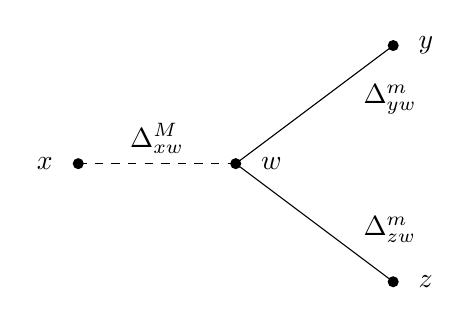
\begin{tikzpicture}[baseline=(current bounding box.center)]
                \begin{feynman}
                  % Vertex with a label
                  % External legs
                  
                  \vertex[label={[shift={(0.2cm, 0cm)}]right:$w$}] (v) at (0, 0);
                  \vertex[label={[shift={(-0.2cm, 0cm)}]left:$x$}]  (a) at (-2, 0);
                  \vertex[label={[shift={(0.2cm, 0cm)}]right:$y$}]  (b) at (2, 1.5);
                  \vertex[label={[shift={(0.2cm, 0cm)}]right:$z$}]  (c) at (2, -1.5);


                  \fill (v) circle (2pt);
                  \fill (a) circle (2pt);
                  \fill (b) circle (2pt);
                  \fill (c) circle (2pt);

                  
                  % Dashed line
                  \diagram* {
                    (a) -- [dashed, edge label={$\Delta_{xw}^{M}$}] (v) [dot],
                    (v) -- [edge label'={$\Delta_{yw}^{m}$}, near end] (b),
                    (v) -- [edge label={$\Delta_{zw}^{m}$}, near end] (c),
                  };
                \end{feynman}
            \end{tikzpicture}
            \end{center}
    \end{minipage}

    

    \item[(c)]
    \item[(d)]
    \newpage
    \item[(e)]
    % thanks to chat gpt, thiago and sarra for adivces and help counting and drawing the diagrams
    \begin{equation*}
        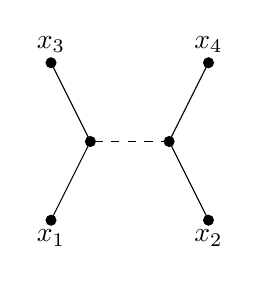
\begin{tikzpicture}[baseline=-\the\dimexpr\fontdimen22\textfont2\relax]
          \begin{feynman}
            % External legs
            \vertex[label={below:$x_1$}] (a) at (-1, -1);
            \vertex[label={below:$x_2$}] (b) at (1, -1);
            \vertex[label={above:$x_3$}] (c) at (-1, 1);
            \vertex[label={above:$x_4$}] (d) at (1, 1);

            \vertex (e) at (-0.5, 0);
            \vertex (f) at (0.5, 0);

            \fill (a) circle (2pt);
            \fill (b) circle (2pt);
            \fill (c) circle (2pt);
            \fill (d) circle (2pt);
            \fill (e) circle (2pt);
            \fill (f) circle (2pt);
      
            \diagram* {
              (a) -- (e),
              (b) -- (f),
              (e) -- (c),
              (f) -- (d),
              (f) -- [dashed] (e),
            };
          \end{feynman}
        \end{tikzpicture}
        +
        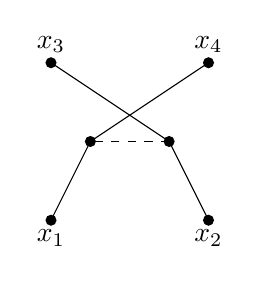
\begin{tikzpicture}[baseline=-\the\dimexpr\fontdimen22\textfont2\relax]
            \begin{feynman}
              % External legs
              \vertex[label={below:$x_1$}] (a) at (-1, -1);
              \vertex[label={below:$x_2$}] (b) at (1, -1);
              \vertex[label={above:$x_3$}] (c) at (-1, 1);
              \vertex[label={above:$x_4$}] (d) at (1, 1);
  
              \vertex (e) at (-0.5, 0);
              \vertex (f) at (0.5, 0);
  
              \fill (a) circle (2pt);
              \fill (b) circle (2pt);
              \fill (c) circle (2pt);
              \fill (d) circle (2pt);
              \fill (e) circle (2pt);
              \fill (f) circle (2pt);
        
              \diagram* {
                (a) -- (e),
                (b) -- (f),
                (e) -- (d),
                (f) -- (c),
                (f) -- [dashed] (e),
              };
            \end{feynman}
          \end{tikzpicture}
          +
          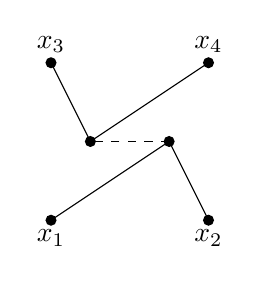
\begin{tikzpicture}[baseline=-\the\dimexpr\fontdimen22\textfont2\relax]
            \begin{feynman}
              % External legs
              \vertex[label={below:$x_1$}] (a) at (-1, -1);
              \vertex[label={below:$x_2$}] (b) at (1, -1);
              \vertex[label={above:$x_3$}] (c) at (-1, 1);
              \vertex[label={above:$x_4$}] (d) at (1, 1);
  
              \vertex (e) at (-0.5, 0);
              \vertex (f) at (0.5, 0);
  
              \fill (a) circle (2pt);
              \fill (b) circle (2pt);
              \fill (c) circle (2pt);
              \fill (d) circle (2pt);
              \fill (e) circle (2pt);
              \fill (f) circle (2pt);
        
              \diagram* {
                (c) -- (e),
                (b) -- (f),
                (e) -- (d),
                (f) -- (a),
                (f) -- [dashed] (e),
              };
            \end{feynman}
          \end{tikzpicture}
    \end{equation*}
    \begin{equation*}
          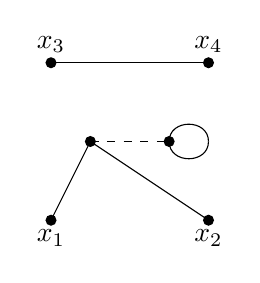
\begin{tikzpicture}[baseline=-\the\dimexpr\fontdimen22\textfont2\relax]
            \begin{feynman}
              % External legs
              \vertex[label={below:$x_1$}] (a) at (-1, -1);
              \vertex[label={below:$x_2$}] (b) at (1, -1);
              \vertex[label={above:$x_3$}] (c) at (-1, 1);
              \vertex[label={above:$x_4$}] (d) at (1, 1);
  
              \vertex (e) at (-0.5, 0);
              \vertex (f) at (0.5, 0);
              \vertex (l) at (1, 0);
  
              \fill (a) circle (2pt);
              \fill (b) circle (2pt);
              \fill (c) circle (2pt);
              \fill (d) circle (2pt);
              \fill (e) circle (2pt);
              \fill (f) circle (2pt);
        
              \diagram* {
                (a) -- (e),
                (b) -- (e),
                (c) -- (d),
                (e) -- [dashed] (f) -- [half left] (l) -- [half left] (f),
              };
            \end{feynman}
          \end{tikzpicture}
          +
          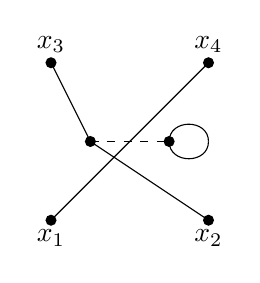
\begin{tikzpicture}[baseline=-\the\dimexpr\fontdimen22\textfont2\relax]
            \begin{feynman}
              % External legs
              \vertex[label={below:$x_1$}] (a) at (-1, -1);
              \vertex[label={below:$x_2$}] (b) at (1, -1);
              \vertex[label={above:$x_3$}] (c) at (-1, 1);
              \vertex[label={above:$x_4$}] (d) at (1, 1);
  
              \vertex (e) at (-0.5, 0);
              \vertex (f) at (0.5, 0);
              \vertex (l) at (1, 0);
  
              \fill (a) circle (2pt);
              \fill (b) circle (2pt);
              \fill (c) circle (2pt);
              \fill (d) circle (2pt);
              \fill (e) circle (2pt);
              \fill (f) circle (2pt);
        
              \diagram* {
                (c) -- (e),
                (b) -- (e),
                (a) -- (d),
                (e) -- [dashed] (f) -- [half left] (l) -- [half left] (f),
              };
            \end{feynman}
          \end{tikzpicture}
          +
          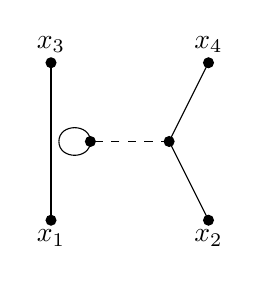
\begin{tikzpicture}[baseline=-\the\dimexpr\fontdimen22\textfont2\relax]
            \begin{feynman}
              % External legs
              \vertex[label={below:$x_1$}] (a) at (-1, -1);
              \vertex[label={below:$x_2$}] (b) at (1, -1);
              \vertex[label={above:$x_3$}] (c) at (-1, 1);
              \vertex[label={above:$x_4$}] (d) at (1, 1);
  
              \vertex (e) at (-0.5, 0);
              \vertex (f) at (0.5, 0);
              \vertex (l) at (-0.9, 0);
  
              \fill (a) circle (2pt);
              \fill (b) circle (2pt);
              \fill (c) circle (2pt);
              \fill (d) circle (2pt);
              \fill (e) circle (2pt);
              \fill (f) circle (2pt);
        
              \diagram* {
                (d) -- (f),
                (a) -- (c),
                (b) -- (f),
                (f) -- [dashed] (e) -- [half left] (l) -- [half left] (e),
              };
            \end{feynman}
          \end{tikzpicture}
          +
          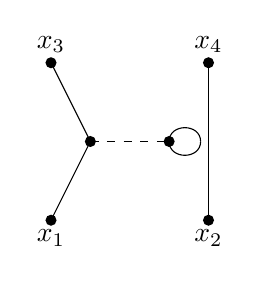
\begin{tikzpicture}[baseline=-\the\dimexpr\fontdimen22\textfont2\relax]
            \begin{feynman}
              % External legs
              \vertex[label={below:$x_1$}] (a) at (-1, -1);
              \vertex[label={below:$x_2$}] (b) at (1, -1);
              \vertex[label={above:$x_3$}] (c) at (-1, 1);
              \vertex[label={above:$x_4$}] (d) at (1, 1);
  
              \vertex (e) at (-0.5, 0);
              \vertex (f) at (0.5, 0);
              \vertex (l) at (0.9, 0);
  
              \fill (a) circle (2pt);
              \fill (b) circle (2pt);
              \fill (c) circle (2pt);
              \fill (d) circle (2pt);
              \fill (e) circle (2pt);
              \fill (f) circle (2pt);
        
              \diagram* {
                (c) -- (e),
                (b) -- (d),
                (a) -- (e),
                (e) -- [dashed] (f) -- [half left] (l) -- [half left] (f),
              };
            \end{feynman}
          \end{tikzpicture}
          +
          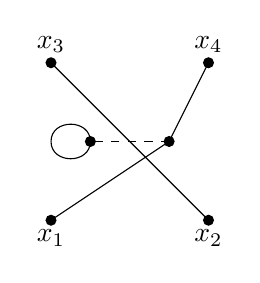
\begin{tikzpicture}[baseline=-\the\dimexpr\fontdimen22\textfont2\relax]
            \begin{feynman}
              % External legs
              \vertex[label={below:$x_1$}] (a) at (-1, -1);
              \vertex[label={below:$x_2$}] (b) at (1, -1);
              \vertex[label={above:$x_3$}] (c) at (-1, 1);
              \vertex[label={above:$x_4$}] (d) at (1, 1);
  
              \vertex (e) at (-0.5, 0);
              \vertex (f) at (0.5, 0);
              \vertex (l) at (-1, 0);
  
              \fill (a) circle (2pt);
              \fill (b) circle (2pt);
              \fill (c) circle (2pt);
              \fill (d) circle (2pt);
              \fill (e) circle (2pt);
              \fill (f) circle (2pt);
        
              \diagram* {
                (d) -- (f),
                (a) -- (f),
                (b) -- (c),
                (f) -- [dashed] (e) -- [half left] (l) -- [half left] (e),
              };
            \end{feynman}
          \end{tikzpicture}
          +
          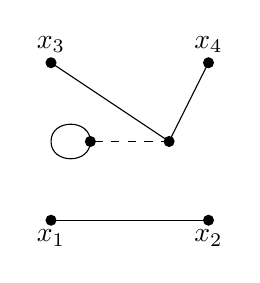
\begin{tikzpicture}[baseline=-\the\dimexpr\fontdimen22\textfont2\relax]
            \begin{feynman}
              % External legs
              \vertex[label={below:$x_1$}] (a) at (-1, -1);
              \vertex[label={below:$x_2$}] (b) at (1, -1);
              \vertex[label={above:$x_3$}] (c) at (-1, 1);
              \vertex[label={above:$x_4$}] (d) at (1, 1);
  
              \vertex (e) at (-0.5, 0);
              \vertex (f) at (0.5, 0);
              \vertex (l) at (-1, 0);
  
              \fill (a) circle (2pt);
              \fill (b) circle (2pt);
              \fill (c) circle (2pt);
              \fill (d) circle (2pt);
              \fill (e) circle (2pt);
              \fill (f) circle (2pt);
        
              \diagram* {
                (a) -- (b),
                (c) -- (f),
                (d) -- (f),
                (f) -- [dashed] (e) -- [half left] (l) -- [half left] (e),
              };
            \end{feynman}
          \end{tikzpicture}
    \end{equation*}
    \begin{equation*}
        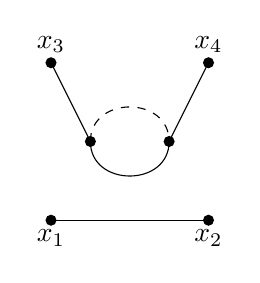
\begin{tikzpicture}[baseline=-\the\dimexpr\fontdimen22\textfont2\relax]
            \begin{feynman}
              % External legs
              \vertex[label={below:$x_1$}] (a) at (-1, -1);
              \vertex[label={below:$x_2$}] (b) at (1, -1);
              \vertex[label={above:$x_3$}] (c) at (-1, 1);
              \vertex[label={above:$x_4$}] (d) at (1, 1);
  
              \vertex (e) at (-0.5, 0);
              \vertex (f) at (0.5, 0);
              \vertex (l) at (0.9, 0);
  
              \fill (a) circle (2pt);
              \fill (b) circle (2pt);
              \fill (c) circle (2pt);
              \fill (d) circle (2pt);
              \fill (e) circle (2pt);
              \fill (f) circle (2pt);
        
              \diagram* {
                (b) -- (a),
                (c) -- (e),
                (e) -- [dashed, half left] (f) -- [half left] (e),
                (f) -- (d),
              };
            \end{feynman}
          \end{tikzpicture}
          +
        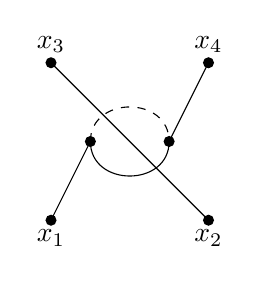
\begin{tikzpicture}[baseline=-\the\dimexpr\fontdimen22\textfont2\relax]
            \begin{feynman}
              % External legs
              \vertex[label={below:$x_1$}] (a) at (-1, -1);
              \vertex[label={below:$x_2$}] (b) at (1, -1);
              \vertex[label={above:$x_3$}] (c) at (-1, 1);
              \vertex[label={above:$x_4$}] (d) at (1, 1);
  
              \vertex (e) at (-0.5, 0);
              \vertex (f) at (0.5, 0);
              \vertex (l) at (0.9, 0);
  
              \fill (a) circle (2pt);
              \fill (b) circle (2pt);
              \fill (c) circle (2pt);
              \fill (d) circle (2pt);
              \fill (e) circle (2pt);
              \fill (f) circle (2pt);
        
              \diagram* {
                (b) -- (c),
                (a) -- (e),
                (e) -- [dashed, half left] (f) -- [half left] (e),
                (f) -- (d),
              };
            \end{feynman}
        \end{tikzpicture}
        + 
        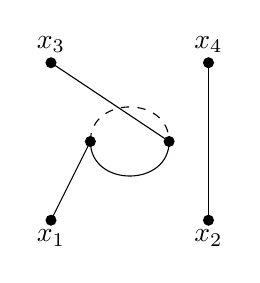
\begin{tikzpicture}[baseline=-\the\dimexpr\fontdimen22\textfont2\relax]
            \begin{feynman}
              % External legs
              \vertex[label={below:$x_1$}] (a) at (-1, -1);
              \vertex[label={below:$x_2$}] (b) at (1, -1);
              \vertex[label={above:$x_3$}] (c) at (-1, 1);
              \vertex[label={above:$x_4$}] (d) at (1, 1);
  
              \vertex (e) at (-0.5, 0);
              \vertex (f) at (0.5, 0);
              \vertex (l) at (0.9, 0);
  
              \fill (a) circle (2pt);
              \fill (b) circle (2pt);
              \fill (c) circle (2pt);
              \fill (d) circle (2pt);
              \fill (e) circle (2pt);
              \fill (f) circle (2pt);
        
              \diagram* {
                (b) -- (d),
                (a) -- (e),
                (e) -- [dashed, half left] (f) -- [half left] (e),
                (f) -- (c),
              };
            \end{feynman}
          \end{tikzpicture}
          +
          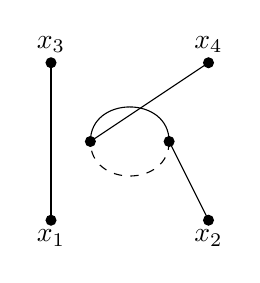
\begin{tikzpicture}[baseline=-\the\dimexpr\fontdimen22\textfont2\relax]
            \begin{feynman}
              % External legs
              \vertex[label={below:$x_1$}] (a) at (-1, -1);
              \vertex[label={below:$x_2$}] (b) at (1, -1);
              \vertex[label={above:$x_3$}] (c) at (-1, 1);
              \vertex[label={above:$x_4$}] (d) at (1, 1);
  
              \vertex (e) at (-0.5, 0);
              \vertex (f) at (0.5, 0);
              \vertex (l) at (0.9, 0);
  
              \fill (a) circle (2pt);
              \fill (b) circle (2pt);
              \fill (c) circle (2pt);
              \fill (d) circle (2pt);
              \fill (e) circle (2pt);
              \fill (f) circle (2pt);
        
              \diagram* {
                (a) -- (c),
                (b) -- (f),
                (f) -- [dashed, half left] (e) -- [half left] (f),
                (e) -- (d),
              };
            \end{feynman}
          \end{tikzpicture}
          +
          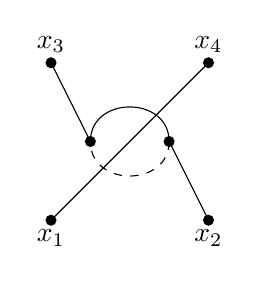
\begin{tikzpicture}[baseline=-\the\dimexpr\fontdimen22\textfont2\relax]
            \begin{feynman}
              % External legs
              \vertex[label={below:$x_1$}] (a) at (-1, -1);
              \vertex[label={below:$x_2$}] (b) at (1, -1);
              \vertex[label={above:$x_3$}] (c) at (-1, 1);
              \vertex[label={above:$x_4$}] (d) at (1, 1);
  
              \vertex (e) at (-0.5, 0);
              \vertex (f) at (0.5, 0);
              \vertex (l) at (0.9, 0);
  
              \fill (a) circle (2pt);
              \fill (b) circle (2pt);
              \fill (c) circle (2pt);
              \fill (d) circle (2pt);
              \fill (e) circle (2pt);
              \fill (f) circle (2pt);
        
              \diagram* {
                (a) -- (d),
                (b) -- (f),
                (f) -- [dashed, half left] (e) -- [half left] (f),
                (e) -- (c),
              };
            \end{feynman}
          \end{tikzpicture}
          +
          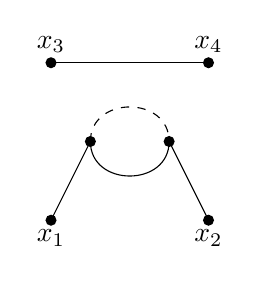
\begin{tikzpicture}[baseline=-\the\dimexpr\fontdimen22\textfont2\relax]
            \begin{feynman}
              % External legs
              \vertex[label={below:$x_1$}] (a) at (-1, -1);
              \vertex[label={below:$x_2$}] (b) at (1, -1);
              \vertex[label={above:$x_3$}] (c) at (-1, 1);
              \vertex[label={above:$x_4$}] (d) at (1, 1);
  
              \vertex (e) at (-0.5, 0);
              \vertex (f) at (0.5, 0);
              \vertex (l) at (0.9, 0);
  
              \fill (a) circle (2pt);
              \fill (b) circle (2pt);
              \fill (c) circle (2pt);
              \fill (d) circle (2pt);
              \fill (e) circle (2pt);
              \fill (f) circle (2pt);
        
              \diagram* {
                (d) -- (c),
                (a) -- (e),
                (e) -- [dashed, half left] (f) -- [half left] (e),
                (f) -- (b),
              };
            \end{feynman}
          \end{tikzpicture}
    \end{equation*}
    \begin{equation*}
        \left[
        \begin{tikzpicture}[baseline=-\the\dimexpr\fontdimen22\textfont2\relax]
            \begin{feynman}
              % External legs
              \vertex[label={below:$x_1$}] (a) at (-1, -1);
              \vertex[label={below:$x_2$}] (b) at (1, -1);
              \vertex[label={above:$x_3$}] (c) at (-1, 1);
              \vertex[label={above:$x_4$}] (d) at (1, 1);
  
              
  
              \fill (a) circle (2pt);
              \fill (b) circle (2pt);
              \fill (c) circle (2pt);
              \fill (d) circle (2pt);
        
              \diagram* {
                (d) -- (c),
                (a) -- (b),
              };
            \end{feynman}
          \end{tikzpicture}
          +
          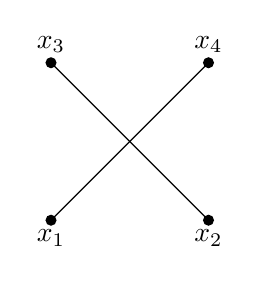
\begin{tikzpicture}[baseline=-\the\dimexpr\fontdimen22\textfont2\relax]
            \begin{feynman}
              % External legs
              \vertex[label={below:$x_1$}] (a) at (-1, -1);
              \vertex[label={below:$x_2$}] (b) at (1, -1);
              \vertex[label={above:$x_3$}] (c) at (-1, 1);
              \vertex[label={above:$x_4$}] (d) at (1, 1);
  
              
  
              \fill (a) circle (2pt);
              \fill (b) circle (2pt);
              \fill (c) circle (2pt);
              \fill (d) circle (2pt);
        
              \diagram* {
                (d) -- (a),
                (b) -- (c),
              };
            \end{feynman}
          \end{tikzpicture}
          +
          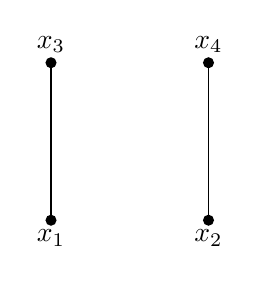
\begin{tikzpicture}[baseline=-\the\dimexpr\fontdimen22\textfont2\relax]
            \begin{feynman}
              % External legs
              \vertex[label={below:$x_1$}] (a) at (-1, -1);
              \vertex[label={below:$x_2$}] (b) at (1, -1);
              \vertex[label={above:$x_3$}] (c) at (-1, 1);
              \vertex[label={above:$x_4$}] (d) at (1, 1);
  
              
  
              \fill (a) circle (2pt);
              \fill (b) circle (2pt);
              \fill (c) circle (2pt);
              \fill (d) circle (2pt);
        
              \diagram* {
                (d) -- (b),
                (a) -- (c),
              };
            \end{feynman}
          \end{tikzpicture}
        \right]
        \times 
        \left[
        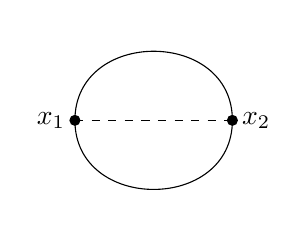
\begin{tikzpicture}[baseline=-\the\dimexpr\fontdimen22\textfont2\relax]
            \begin{feynman}
              % External legs
              \vertex[label={left:$x_1$}] (a) at (-1, 0);
              \vertex[label={right:$x_2$}] (b) at (1, 0);
  
              \fill (a) circle (2pt);
              \fill (b) circle (2pt);
        
              \diagram* {
                (a) -- [half left] (b) -- [half left] (a),
                (a) -- [dashed] (b),
              };
            \end{feynman}
          \end{tikzpicture}
          +
          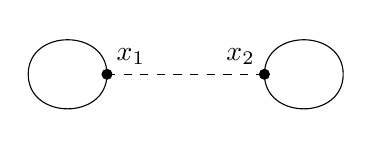
\begin{tikzpicture}[baseline=-\the\dimexpr\fontdimen22\textfont2\relax]
            \begin{feynman}
              % External legs
              \vertex[label={above right:$x_1$}] (a) at (-1, 0);
              \vertex[label={above left:$x_2$}] (b) at (1, 0);
              \vertex (l1) at (2, 0);
              \vertex (l2) at (-2, 0);
  
              \fill (a) circle (2pt);
              \fill (b) circle (2pt);
        
              \diagram* {
                (a) -- [half left] (l2) -- [half left] (a),
                (b) -- [half left] (l1) -- [half left] (b),
                (a) -- [dashed] (b),
              };
            \end{feynman}
          \end{tikzpicture}
        \right]
    \end{equation*}
    \item[(f)]
    \item[(g)]
    \item[(h)]  
\end{enumerate}



\section{Acknowledgement}


% References
\makereferences
%-------------------------------------------------------


%%%%%%%%%%%%%%%%%%%%%%%%
% Terminer le document %
%%%%%%%%%%%%%%%%%%%%%%%%
\end{document}